% main.tex -- Advionics report, EUROAVIA Ideathon 2026
% Compile in this folder:  latexmk -lualatex main.tex
% Numbers: cases/case_10_par_hybrid_cue/outputs/{result.md,validation.json},
%          submission/report_build/report_numbers.json. Figures: report_build/report_figures.py.
\documentclass{ideathon2026}
\usepackage{amsmath}
\usepackage{tikz}
\usetikzlibrary{arrows.meta,positioning}

% ---- cover page -------------------------------------------------------
\reporttitle{Automated PAR Cue}
\reportsubtitle{Radar data to pilot guidance, without a controller}
\teamname{Team Beetiful}
\challenge{EUROAVIA Ideathon 2026 -- Advionics challenge\newline
  {\fontsize{11bp}{16bp}\selectfont Ayberk Demirkanat, Rabia Nur Toprak,\newline
  Zeynep Simge Aydın, Kaan Çınıçev}}
% small team logo on the white part of the cover, drawn after the cover image
\makeatletter
\g@addto@macro\ideathon@drawcover{%
  \put(432,-505){
\includegraphics[width=92bp]{figures/team_logo.png}}}
\makeatother

\paragraphspacing{4.5bp}

\begin{document}

\makecover
\tableofcontents

\section{Introduction}
A Precision Approach Radar (PAR) shows a controller the distance, lateral offset and height offset of an aircraft on final
approach. The controller reads these values and talks the pilot down in low visibility \cite{skybrary,aim,afman}. FAA Order
JO 7110.65BB asks for one transmission about every 5 s \cite{jo}. Advionics asks us to automate this chain with no controller. Radar data goes
in, and heading and glidepath corrections go out as a clear cue to the pilot \cite{brief}.

We chose the HYBRID direction (Figure~\ref{fig:flow}). A display updates with every radar plot, and voice speaks only for
important changes. A 5 s voice rhythm is a limit of the human talk-down, and a display does not block the radio. The words are
FAA words, so a pilot who knows a PAR talk-down can read them at once.

We assume a working radar, an aircraft established on final and a decision height (DH) of 200 ft. This is an educational
concept on simulated and recorded data. It is not approved or ready for operational flight use.

\begin{figure}[b]
\centering
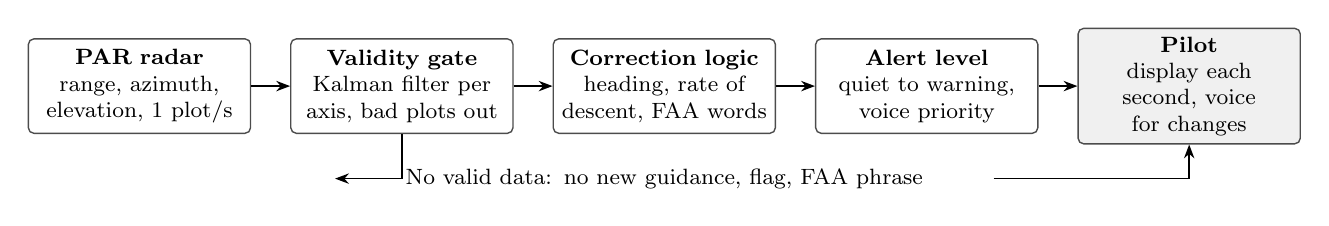
\begin{tikzpicture}[font=\fontsize{7.5bp}{9.5bp}\selectfont,
  box/.style={draw=black!70, line width=.5pt, rounded corners=2pt, minimum height=34bp, text width=74bp, align=center, inner sep=3pt},
  arr/.style={-{Stealth[length=5pt]}, line width=.6pt}]
  \node[box] (a) {\textbf{PAR radar}\\range, azimuth, elevation, 1 plot/s};
  \node[box, right=14bp of a] (b) {\textbf{Validity gate}\\Kalman filter per axis, bad plots out};
  \node[box, right=14bp of b] (c) {\textbf{Correction logic}\\heading, rate of descent, FAA words};
  \node[box, right=14bp of c] (d) {\textbf{Alert level}\\quiet to warning, voice priority};
  \node[box, right=14bp of d, fill=black!6] (e) {\textbf{Pilot}\\display each second, voice for changes};
  \draw[arr] (a) -- (b); \draw[arr] (b) -- (c); \draw[arr] (c) -- (d); \draw[arr] (d) -- (e);
  \node[below=9bp of c, text width=230bp, align=center] (f) {No valid data: no new guidance, flag, FAA phrase};
  \draw[arr] (b.south) |- (f.west); \draw[arr] (f.east) -| (e.south);
\end{tikzpicture}
\caption{Radar to pilot flow. The link from the ground to the cockpit is assumed.}
\label{fig:flow}
\end{figure}

\section{Synthetic data}
\subsection{Purpose and limits}
We found no measured PAR plots. A recorded track also cannot test the cue, because a recorded aircraft does not react to it.
So we built a closed loop: radar plots feed the cue, a pilot model flies the cue, and the aircraft moves. Faults start at a
known time and repeat with the same seed. The model tests the logic. It does not predict how a real pilot performs.

\subsection{Basic equations}
Radar error uses the ICAO Annex 10 limits \cite{icao10}. $R$ is the distance from the antenna; $y$ and $z$ are the lateral and
vertical deviation. We assume that $1\sigma$ is half of the limit:
\begin{equation}
\sigma_{\mathrm{az}} = \tfrac12\max(0.006R + 0.1|y|,\ 9\,\mathrm{m}),\qquad
\sigma_{\mathrm{el}} = \tfrac12\max(0.004R + 0.1|z|,\ 6\,\mathrm{m}).
\end{equation}
The aircraft is a point mass with airspeed $V$, heading $\psi$, sink rate $s$, crosswind $W_c$ and vertical gust $w$:
\begin{equation}
\dot y = V\sin\psi + W_c,\qquad \dot z = w - s.
\end{equation}
Wind grows with height $h$ from its 20 ft value $W_{20}$ ($h$ and $z_0 = 0.15$ in ft). Gusts follow the low-altitude Dryden form
with turbulence level $W_t$, 15 kt when light \cite{dryden,shear}:
\begin{equation}
W(h) = W_{20}\,\frac{\ln(h/z_0)}{\ln(20/z_0)},\qquad \sigma_w = 0.1\,W_t.
\end{equation}

\begin{table}[tb]
\caption{The model covers the full chain at low order. Simulation results hold only inside this scope.}
\label{tab:scope}
\begin{tabular}{L{62bp}L{246bp}L{190.9bp}}
\toprule
\thead{Element} & \thead{In the model} & \thead{Left out}\\
\midrule
Radar geometry & Antenna 915 m back and 120 m aside, 1 plot/s, 9 NM, 20° sector \cite{icao10} & Beam scan, clutter, rain\\
Radar error & Annex 10 limits, half of the variance correlated over 5 s; 0.05° multipath term [both assumed] & Measured PAR error, real terrain\\
Plot loss & 95 \% detection, 90 \% as a test case & Long burst losses\\
Wind & Log-law profile, crosswind up to 10 m/s \cite{shear} & Microburst, wind-shear events\\
Turbulence & Dryden, light (15 kt) and moderate (30 kt) \cite{dryden} & Severe turbulence, wake\\
Aircraft & Point mass, 130 kt C-130H or 137 kt A320 \cite{eurocontrol}, 4 s lag & 6-DOF dynamics, speed change, flare\\
Pilot & 2 s reaction [no PAR source; analogy from EGPWS response], 1.5°/s turns, height loop 0.25 rad/s \cite{nasa}, 1° pitch limit & Workload, fatigue, startle, pilot error\\
Faults, link & Delay, jump, invalid flag, radar stop, link on or off & Spoofing, link latency, bit errors\\
Procedure & Starts on final at 5 NM & Vectors, begin-descent call, mile calls by voice\\
\bottomrule
\end{tabular}
\end{table}

\subsection{Closed-loop result}
The test follows the brief. The aircraft starts at 5 NM, 150 m right and 30 m high, with 3 m/s crosswind and light turbulence. We
ran 100 seeds. The first pilot model flies a rounded heading target that changes at most every 5 s, as a controller's heading does. The second flies
the marker into the display ring (Section 4).

\begin{figure}[tb]
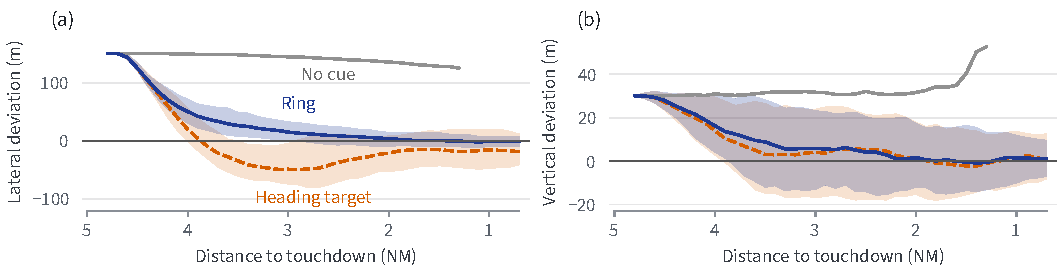
\includegraphics[width=\linewidth]{figures/F2_return_to_path.pdf}
\caption{Both cue laws remove the start offset. The ring also removes the overshoot. Lines are medians and bands are 5 to 95 \% of 100 runs. The no-cue line ends where most runs leave the limits.}
\label{fig:return}
\end{figure}

With the heading target, 99 of 100 runs reach DH, with a 95 \% error of 37 m lateral and 11 m vertical. With the ring, 99 of 100
reach DH with 11 m and 9 m. That ring pilot reads drift from the marker with no error, so 11 m is a best case. With no cue, 1 of
100 reaches DH. The heading target gives 95 of 100 with a 4 s reaction and 96 at 90 \% detection. It gives 100 with a radar twice as good
and 77 in moderate turbulence (ring: 76). A 300 m start at 5 m/s crosswind gives 65.

\section{Test on recorded data}
\subsection{Zurich: agreement and replay}
We used 1000 recorded tracks on Zurich runway 14 (ADS-B, October and November 2019) \cite{figshare}. They are the first 1000 tracks
that passed our filter, not a random sample. For this comparison the simulation starts on the path, with no steady wind, at A320
speed. Speed is an input (137 kt; recorded median 141 kt). Sink rate is a result: 726 ft/min against 747 ft/min recorded, with 5 to
95 \% ranges of 640--849 and 667--842 ft/min.

\begin{figure}[tb]
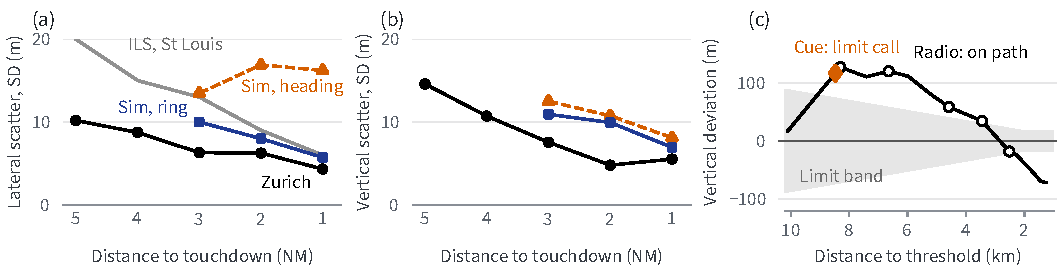
\includegraphics[width=\linewidth]{figures/F3_real_data.pdf}
\caption{Simulated scatter is wider than real scatter. (a, b) Scatter between flights: 1000 recorded tracks, 100 simulated runs and published ILS data \cite{hall}. (c) Smolensk 2010: track from 13 report points, $\pm$0.5° limit, the five radio position calls (circles) and the first limit call of the cue in replay (diamond).}
\label{fig:real}
\end{figure}

With the ring, simulated lateral scatter is 1.3 to 1.6 times the recorded value, and vertical scatter 1.3 to 2.1 times. With the
heading target, lateral scatter is 2.1 to 3.7 times the recorded value. A perfect radar does not reduce it (13 to 18 m), so the cause
is the heading steps. A perfect radar does reduce vertical scatter to 4 to 5 m, so PAR accuracy sets the vertical result. These
aircraft flew ILS, and the simulated aircraft flew the cue, so the two scatters are not a like-for-like test. We also removed one
height constant per flight, because ADS-B height differs by aircraft. Recorded vertical scatter is therefore a lower bound.

Each track then went through the Annex 10 radar model and the cue. The aircraft did not react to the cue. No pilot saw it. Of 1000
tracks, 985 stayed quiet, 5 reached advise, 4 caution and 6 warning. On 98.5 \% of tracks the cue gave no guidance voice, and 275
tracks ended before DH. We did not check whether the 6 warnings were real excursions. At 90 \% detection, 8 tracks ended in a false
RADAR LOST.

Recorded data changed the design. With no noise margin and no frame count, the closure flag fired on 397 of 1000 tracks. Simulation
had not shown this. With both it fires on 6. This is not an independent result, because we tuned the flag on the first 300 of these
tracks and on the Smolensk track. Of 66 go-arounds labelled on this runway \cite{zenodo}, we could cut 22 out of the tracks. The cue
spoke before the climb in 11, with a median lead of 15 s.

\subsection{Smolensk 2010: a radar talk-down}
This is the one event we found with a radar talk-down and stated deviations \cite{smolensk}. We use deviations and calls only, with no
finding on blame. The radio said ``on course, on glide path'' five times outside the on-path band. The first correction came 5.5 s
before the first tree strike. In replay, our limit call would have come 88.5 s before it (median, 200 of 200 noisy runs). With the
limit switched off, ``Coming down rapidly'' would have come 16.5 s before it, in 167 of 200 runs. If the radar itself was wrong, as
the report suspects, the cue would inherit the error.

\section{The cue on the display}
\subsection{Marker logic}
ICAO treats the axes differently \cite{icao4444}. In azimuth the pilot gets a heading. In elevation the pilot corrects from position
information. The law follows this and uses radar position only. Three designs with a radar-derived rate failed
(0 of 100 runs reached DH), because a rate from 1 Hz plots is too noisy. With ground speed $V_g$, range $r$ and path angle $\gamma$,
the look-ahead time $T$, the aim track $\chi_r$ and the aim sink rate $s_r$ are:
\begin{equation}
T = \min\!\Big(20\,\mathrm{s},\ \max\big(\tfrac{r}{2V_g},\ 8\,\mathrm{s}\big)\Big),\quad
\chi_r = -\arctan\frac{y}{V_g T},\quad
s_r = V_g\tan\gamma + \frac{z}{T}.
\end{equation}
Corrections are capped at 10° (5° inside 3 NM) and 1.2 m/s. We use symbols that pilots already know (Figure~\ref{fig:display}):
\begin{itemize}
\item \textbf{Diamonds: where the path is.} Scales as on an ILS, 1 dot = 1.25° lateral and 0.35° vertical.
\item \textbf{Marker: where you go.} Real track and flight path angle from aircraft sensors, not from the radar. Wind needs no term.
\item \textbf{Ring: where to go.} The point on the path $T$ seconds ahead, at $\chi_r$ and $s_r$. It turns green with the marker inside.
\end{itemize}
With the marker in the ring, $\dot y = -y/T$, so the offset decays with time constant $T$. An aircraft with no flight path marker cannot
use the ring. It can use the diamonds, the heading and the FAA words.

\begin{figure}[tb]
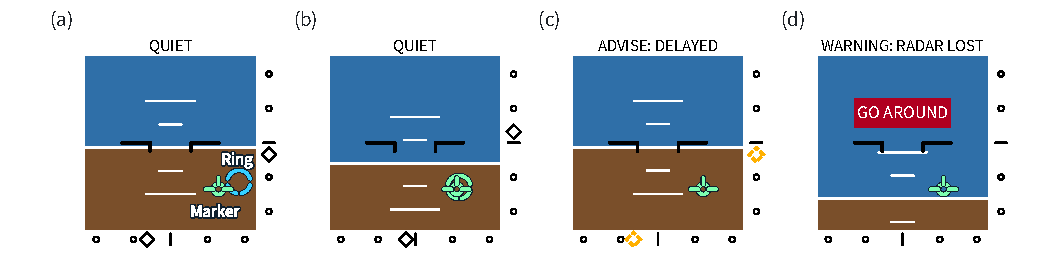
\includegraphics[width=\linewidth]{figures/F4_display.pdf}
\caption{The symbols show the state before the pilot reads any text. (a) Off path: marker outside the ring. (b) On path: marker in the green ring. (c) Data 4 s old: hollow diamonds, no ring. (d) Radar lost: no diamonds, no ring. Replay frames; horizon position is schematic.}
\label{fig:display}
\end{figure}

\subsection{Alert levels and voice}
Below 1 dot the level is quiet. At 1 dot it is advise (stable approach limit \cite{fsf}). At 1.3 dots it is caution (EGPWS Mode 5 soft
alert \cite{egpws}). In a missed approach state it is warning. The limits $\pm$0.5° and $\pm$2° come from one report \cite{smolensk}. The FAA
prints no number, and a real system takes them per runway. A call repeats only for 20 \% more deviation. The cue ranks below every
aircraft alert \cite{faahf}. With an aircraft alert sounding, the cue is silent and a warning waits. With a transmission on, a routine
call is dropped. The display never waits. Voice repeats the display words \cite{ac}.

\section{When data goes wrong}
With no valid data, the cue gives no new guidance and no extrapolation (Table~\ref{tab:faults}). A missed approach call is the reason,
then the condition \cite{jo}. The pilot decides. The short GO AROUND flag on the mock-up points to that call. None of these calls applies
after DH.

\begin{table}[tb]
\caption{Each fault has one display state and one call. The pilot never sees old data without a mark. 3 s and 4 NM are UK values \cite{ra3291}; 5 s is the longest ICAO silence \cite{icao4444} and the FAA lost communications interval.}
\label{tab:faults}
\begin{tabular}{L{70bp}L{52bp}L{108bp}L{204bp}L{64.9bp}}
\toprule
\thead{Event} & \thead{Told after} & \thead{Display} & \thead{Voice} & \thead{Basis}\\
\midrule
Plots late & 3 s & Diamonds hollow, ring off, no new heading & ``Radar data delayed'' & RA 3291\\
Bad plots (jump, invalid) & 2 plots & Diamond of that axis off, back after 3 good plots & ``Radar data invalid'' & Design value\\
Radar contact lost & 3 s (5 s beyond 4 NM) & All guidance off, latched & ``Radar contact lost. If runway or approach lights not in sight, execute missed approach.'' & JO 5-10-14c\\
Elevation failed & 2 plots & All guidance off, latched & ``No glidepath information available. If runway\ldots'' & JO 5-12-10\\
Outside limits & 3 s & All guidance off, latched & ``Too low for safe approach. If runway\ldots'' & JO 5-10-14a\\
Link silent & 5 s & All guidance off & ``Guidance link lost. Apply lost communications procedure.'' Not a missed approach & JO 5-10-4\\
Any fault below DH & -- & Diamond off, advisory text & None & JO 5-10-14, 5-12-7\\
\bottomrule
\end{tabular}
\end{table}

In all 100 seeded runs, the cue told a 4 s delay and a radar stop after 3 s. It told a 400 m jump after 1 s in 90 runs. No frame
showed guidance without valid data. The weak point is a wrong but plausible plot. Far out, a jump below 200 m was not caught. Near the
runway, a jump below 150 m was mostly not caught. Such a jump moved the aircraft by up to 66 m (95 \%).

\section{Limits and next step}
No real pilot has flown this cue, so we claim no drop in workload. Voice less often than every 5 s departs from the FAA rhythm and needs
a pilot trial. Radar to cockpit needles is not new: Navy ACLS Mode II does this \cite{fas,jo}. Our work is the logic behind the display:
FAA fault rules, a silent path and a voice that yields to aircraft alerts. We tested it in a replay of 1000 recorded tracks.

For Advionics the airborne change is one display page and one data link, and the radar stays. The work fits its RF, embedded software and
test skills \cite{advionics}. The next step is a pilot-in-the-loop simulator trial. Recorded PAR plots, link latency tests and an
independent height check follow.

% ---- references: extra pages, outside the 5-page limit -----------------
\clearpage
\begin{thebibliography}{99}
\bibitem{brief} Advionics NV, ``Automated Precision Approach Guidance,'' EUROAVIA Ideathon challenge brief, 2026.
\bibitem{jo} Federal Aviation Administration, Order JO 7110.65BB, \emph{Air Traffic Control}, effective 20 Feb. 2025, with Change 1 and 2 (22 Jan. 2026), Ch. 5 Sections 10 and 12. The FAA site refused automated reading, so we read a third-party copy: \url{https://cdn.sprinkle.com/library/pdfs/4dc0aa14-617e-413e-8f42-2642e94301d5.pdf}. Official page: \url{https://www.faa.gov/air_traffic/publications/atpubs/atc_html/chap5_section_12.html}
\bibitem{aim} Federal Aviation Administration, \emph{Aeronautical Information Manual}, para 5-4-11, Radar Approaches. Mirror: \url{https://faraim.org/faa/aim/chapter-5/section-5-4-11.pdf}
\bibitem{afman} US Air Force, AFMAN 11-217, \emph{Flight Operations}, 10 June 2019, para 21.8, Radar Approaches.
\bibitem{ac} Federal Aviation Administration, Advisory Circular AC 25.1322-1, \emph{Flightcrew Alerting}, 13 Dec. 2010.
\bibitem{faahf} Federal Aviation Administration, \emph{Human Factors Considerations in the Design and Evaluation of Flight Deck Displays and Controls}, Section 4.3, Alert Functional Elements, Nov. 2013, Chg 1. Table 4.3.1 reproduces TSO-C151c Table 4-2.
\bibitem{skybrary} SKYbrary, ``Precision Approach Radar (PAR).'' \url{https://skybrary.aero/articles/precision-approach-radar-par}
\bibitem{icao10} ICAO, Annex 10, Vol. I, \emph{Radio Navigation Aids}, 7th ed., July 2018, Section 3.2.3. \url{https://ffac.ch/wp-content/uploads/2020/09/ICAO-Annex-10-Aeronautical-Telecommunications-Vol-I-Radio-Navigation-Aids.pdf}
\bibitem{icao4444} ICAO, Doc 4444, \emph{PANS-ATM}, 16th ed., 2016, Section 8.9.7. \url{https://www.bazl.admin.ch/dam/it/sd-web/jMIWMg9YgaoW/4444_cons_en.pdf}
\bibitem{ra3291} UK Military Aviation Authority, RA 3291 Issue 4, 2025. \url{https://assets.publishing.service.gov.uk/media/68db8f9ac487360cc70c9eea/RA3291_Issue_4.pdf}
\bibitem{dryden} MathWorks, ``Dryden Wind Turbulence Model (Continuous),'' citing MIL-F-8785C. \url{https://www.mathworks.com/help/aeroblks/drydenwindturbulencemodelcontinuous.html}
\bibitem{shear} MathWorks, ``Wind Shear Model,'' citing MIL-F-8785C. \url{https://www.mathworks.com/help/aeroblks/windshearmodel.html}
\bibitem{eurocontrol} EUROCONTROL, Aircraft Performance Database, A320. \url{https://learningzone.eurocontrol.int/ilp/customs/ATCPFDB/details.aspx?ICAO=A320}
\bibitem{nasa} D. Weir, D. McRuer, NASA CR-2019, 1972. \url{https://ntrs.nasa.gov/api/citations/19720016437/downloads/19720016437.pdf}
\bibitem{figshare} ``Reference data sets for detection and identification of significant events in historical aircraft trajectory data,'' Figshare, MIT licence, doi:10.6084/m9.figshare.11406735.v1.
\bibitem{zenodo} ``Large Landing Trajectory Data Set for Go-Around Analysis,'' Zenodo, CC BY 4.0, doi:10.5281/zenodo.7148117.
\bibitem{hall} Hall and Soares, US DOT Volpe, DASC 2008, Table 4. \url{https://rosap.ntl.bts.gov/view/dot/9095/dot_9095_DS1.pdf}
\bibitem{smolensk} Committee for Investigation of National Aviation Accidents (Poland), Final Report 192/2010/11, Tu-154M 101, pp. 13--15, 214--216, 253--271. English information copy: \url{https://doc.rmf.pl/rmf_fm/store/rkm_en.pdf}
\bibitem{fsf} Flight Safety Foundation, ALAR Briefing Note 7.1, Stabilized Approach. \url{https://skybrary.aero/sites/default/files/bookshelf/864.pdf}
\bibitem{egpws} Honeywell, MK V and MK VII EGPWS Pilot Guide, 060-4241-000 Rev. D, Mar. 2000. \url{https://lso.fe.uni-lj.si/literatura/Razno/Avionika/radar/EGPWS.pdf}
\bibitem{fas} Federation of American Scientists, AN/SPN-46. \url{https://man.fas.org/dod-101/sys/ship/weaps/an-spn-46.htm}
\bibitem{advionics} Advionics NV, company web pages. \url{https://advionics.be/}
\end{thebibliography}

\begin{table}[tb]
\caption{FAA rules behind the design. The right column is our use of them.}
\label{tab:faa}
\begin{tabular}{L{86bp}L{226bp}L{186.9bp}}
\toprule
\thead{FAA source} & \thead{What it says} & \thead{What our system does}\\
\midrule
JO 7110.65BB 5-12-4a & Inform on glidepath and on course, and of any deviation; transmit about every 5 s. Words: ON GLIDEPATH, ON COURSE, SLIGHTLY/WELL ABOVE/BELOW GLIDEPATH, SLIGHTLY/WELL LEFT/RIGHT OF COURSE & Same words on the display each second. Voice is rarer on purpose: this departs from the rule and needs a trial\\
JO 7110.65BB 5-12-4b & Trend information as required, with RAPIDLY or SLOWLY & Trend words from a 10 s fit, for words only, never for control\\
JO 7110.65BB 5-10-14 & If the runway environment is not in sight, instruct a missed approach when safety limits are exceeded, position is in doubt, or radar contact is lost or a malfunction suspected. Reason first. Not after DH on a PAR approach & Reason, then ``if runway or approach lights not in sight, execute missed approach''. No such call after DH\\
JO 7110.65BB 5-10-4 & Tell the pilot what to do if radio is lost for 5 s on a PAR final. ACLS Modes I, IA and II: 5 s after loss of data link & Link silent 5 s: the pilot applies the lost communications instruction. Not a missed approach\\
JO 7110.65BB 5-12-7, 5-12-8 & Position information until over the threshold. Below DH it is advisory only (14 CFR 91.175 is the pilot's). Guidance ends over the threshold & Position stays on below DH, marked ADVISORY ONLY, and ends over the threshold\\
JO 7110.65BB 5-12-10 & Elevation failure: stop PAR instructions; take over visually or execute a missed approach. NO GLIDEPATH INFORMATION AVAILABLE & Ends guidance after 2 flagged plots, with this phrase\\
AIM 5-4-11 & A PAR pilot gets headings. For elevation the pilot gets ``slightly'' or ``well'' and adjusts rate of descent. Outside safety limits: missed approach unless the runway environment is in sight & Heading in azimuth, information in elevation. A limit must be exceeded for 3 s before the call\\
AC 25.1322-1 para 12, App. 2 & Design to avoid false and nuisance alerts. Voice should match the displayed text & Silent on the path. Voice uses the display words\\
FAA HF guidance 4.3 (TSO-C151c Table 4-2) & Published priority order of TAWS alerts & The cue ranks below every line of that list\\
\bottomrule
\end{tabular}
\end{table}

\end{document}
